% tikz_proofmap.tex -- fig:proof-map, the cases of the local bound vol(V_c) >= 8.
%   Left: contact configurations, split by the number m of contacts
%   (cor:m22, thm:m23, thm:m24).  Right: a centre within sqrt6 that is not a
%   contact, split by the number |Y| of centres within sqrt6
%   (thm:m23-labelled, thm:count31, thm:count30, prop:C-radial, lem:no-triple,
%   thm:G-pushout, thm:near-contact).  Green boxes are proved, orange boxes are
%   open.
% Test:   python3 tikz_overlap_check.py tikz_proofmap.tex
% Build:  pdflatex tikz_proofmap.tex && pdftoppm -r 500 -png -singlefile tikz_proofmap.pdf ../figures/fig_tikz_proofmap
\documentclass[border=4pt]{standalone}
\usepackage{tikz}
\usetikzlibrary{calc,arrows.meta,positioning}
\usepackage[T1]{fontenc}
\usepackage{lmodern}
\usepackage{amsmath,amssymb}
\DeclareMathOperator{\vol}{vol}
\definecolor{cblue}{HTML}{2A78D6}
\definecolor{corange}{HTML}{EB6834}
\definecolor{caqua}{HTML}{1BAF7A}
\definecolor{cink}{HTML}{0B0B0B}
\definecolor{cink2}{HTML}{52514E}
\definecolor{cink3}{HTML}{8B8A85}
\definecolor{cpanel}{HTML}{F4F3EF}
% tikzcheck.tex -- the hooks of tikz_overlap_check.py, input by the TikZ figures.
% Two ways to name what is checked.
%  - Explicit: \figboxes and \figlabels list named nodes; with \nolabels defined,
%    nodes in the style lbl are drawn invisibly.
%  - Automatic: \autocheck in the preamble gives every node of the picture,
%    pgfplots tick labels included, an alias chk<n>; with \nolabels defined, the
%    text of every node is drawn invisibly and its shape is kept.
% \checkfigure, at the end of the picture, writes the four corners of each
% checked node (so that rotated nodes are measured by their true extent) and
% those of the picture to the log when \checkbboxes is defined.
\tikzset{lbl/.style={}}
\ifdefined\nolabels\tikzset{lbl/.append style={opacity=0}}\fi
\newcount\chknodes
\newcommand\autocheck{% idempotent: a figure with \autocheck may also be run with --auto
  \ifdefined\chkauto\else
  \def\chkauto{}%
  \tikzset{every node/.append style={/utils/exec={\global\advance\chknodes by 1\relax},
                                      alias=chk\the\chknodes}}%
  \ifdefined\nolabels\tikzset{every node/.append style={text opacity=0}}\fi
  \fi}
\makeatletter
% a node counted but never kept (pgfplots typesets some nodes once to measure them)
% has no shape, and is skipped
\newcommand\chkifnode[2]{\pgfutil@ifundefined{pgf@sh@ns@#1}{}{#2}}
\makeatother
\newcommand\chkout[2]{% kind, node
  \path let \p1=(#2.south west), \p2=(#2.north east), \p3=(#2.north west), \p4=(#2.south east)
    in \pgfextra{\typeout{BBOX #1 #2\space\x1\space\y1\space\x2\space\y2\space\x3\space\y3\space\x4\space\y4}};}
\newcommand\checkfigure{%
  \ifdefined\checkbboxes
    \path let \p1=(current bounding box.south west), \p2=(current bounding box.north east)
      in \pgfextra{\typeout{PICBB \x1\space\y1\space\x2\space\y2}};
    \typeout{BORDER 4.0pt}%
    \ifdefined\chkauto
      \edef\chklast{\the\chknodes}%
      \foreach \nm in {1,...,\chklast} {\chkifnode{chk\nm}{\chkout{auto}{chk\nm}}}%
    \else
      \foreach \nm in \figboxes {\chkout{box}{\nm}}%
      \foreach \nm in \figlabels {\chkout{label}{\nm}}%
    \fi
  \fi}
\ifdefined\forceauto\autocheck\fi

\autocheck
\begin{document}
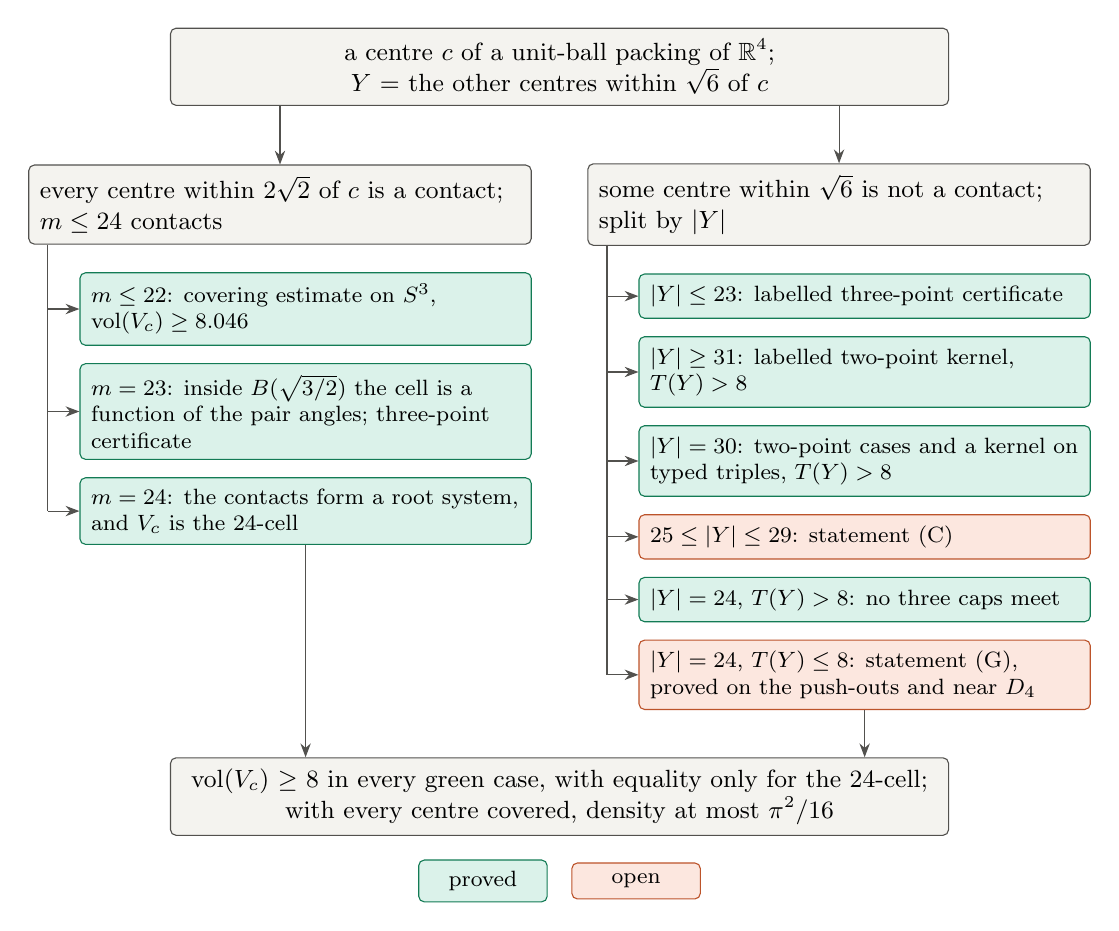
\begin{tikzpicture}[font=\small,
  box/.style={draw=cink2, rounded corners=2pt, align=flush left, inner sep=4pt, text width=#1,
              execute at begin node={\hyphenpenalty=10000\exhyphenpenalty=10000}},
  box/.default=6.1cm,
  head/.style={box=#1, fill=cpanel},
  ok/.style={box=5.45cm, fill=caqua!16, draw=caqua!70!black, font=\footnotesize},
  open/.style={box=5.45cm, fill=corange!16, draw=corange!80!black, font=\footnotesize},
  arr/.style={-{Stealth[length=5pt]}, cink2}]
\node[head=9.6cm, align=center] (root) at (0,0)
  {a centre $c$ of a unit-ball packing of $\mathbb{R}^4$;\\
   $Y$ = the other centres within $\sqrt6$ of $c$};
%% left column
\node[head=6.1cm] (L) at (-3.55,-1.75)
  {every centre within $2\sqrt2$ of $c$ is a contact; $m\le24$ contacts};
\node[ok, anchor=north east] (L1) at ($(L.south east)+(0,-0.35)$)
  {$m\le22$: covering estimate on $S^3$, $\vol(V_c)\ge8.046$};
\node[ok, anchor=north east] (L2) at ($(L1.south east)+(0,-0.22)$)
  {$m=23$: inside $B(\sqrt{3/2})$ the cell is a function of the pair angles; three-point certificate};
\node[ok, anchor=north east] (L3) at ($(L2.south east)+(0,-0.22)$)
  {$m=24$: the contacts form a root system, and $V_c$ is the $24$-cell};
%% right column
\node[head=6.1cm] (R) at (3.55,-1.75)
  {some centre within $\sqrt6$ is not a contact; split by $|Y|$};
\node[ok, anchor=north east] (R1) at ($(R.south east)+(0,-0.35)$) {$|Y|\le23$: labelled three-point certificate};
\node[ok, anchor=north east] (R2) at ($(R1.south east)+(0,-0.22)$) {$|Y|\ge31$: labelled two-point kernel, $T(Y)>8$};
\node[ok, anchor=north east] (R3) at ($(R2.south east)+(0,-0.22)$)
  {$|Y|=30$: two-point cases and a kernel on typed triples, $T(Y)>8$};
\node[open, anchor=north east] (R4) at ($(R3.south east)+(0,-0.22)$) {$25\le|Y|\le29$: statement (C)};
\node[ok, anchor=north east] (R5) at ($(R4.south east)+(0,-0.22)$) {$|Y|=24$, $T(Y)>8$: no three caps meet};
\node[open, anchor=north east] (R6) at ($(R5.south east)+(0,-0.22)$)
  {$|Y|=24$, $T(Y)\le8$: statement (G), proved on the push-outs and near $D_4$};
%% conclusion
\node[head=9.6cm, align=center, anchor=north] (C) at ($(0,0)!(R6.south)!(0,-1)+(0,-0.6)$)
  {$\vol(V_c)\ge8$ in every green case, with equality only for the $24$-cell;\\
   with every centre covered, density at most $\pi^2/16$};
%% arrows
\draw[arr] (root.south) ++(-3.55,0) -- (L.north);
\draw[arr] (root.south) ++(3.55,0) -- (R.north);
\draw[cink2] (L.south west) ++(0.25,0) coordinate (lx) -- (lx |- L3.west);
\foreach \n in {L1,L2,L3} \draw[arr] (lx |- \n.west) -- (\n.west);
\draw[cink2] (R.south west) ++(0.25,0) coordinate (rx) -- (rx |- R6.west);
\foreach \n in {R1,R2,R3,R4,R5,R6} \draw[arr] (rx |- \n.west) -- (\n.west);
\draw[arr] (L3.south) -- (L3.south |- C.north);
\draw[arr] (R6.south) -- (R6.south |- C.north);
%% legend
\node[ok, text width=1.35cm, align=center, anchor=north east] (k1) at ($(C.south)+(-0.15,-0.3)$) {proved};
\node[open, text width=1.35cm, align=center, anchor=west] (k2) at ($(k1.east)+(0.3,0)$) {open};
\checkfigure
\end{tikzpicture}
\end{document}
